\chapter{Conformación de segmentos \ac{tm}-\ac{ic} de integrinas $\alpha$IIb/$\beta$3: Rol del ambiente lipídico}\label{chap:dm}

El ambiente lipídico en el cual se encuentran las proteínas de membrana, puede cambiar sus propiedades biofísicas por diferentes vías, sin embargo se resaltan dos principalmente, variación de las propiedades fisicoquímicas de la bicapa, y através de interacciones moleculares entre las moléculas que la componen \hl{REF}. La presencia de proteínas puede inducir la formación de un ``anillo'' de lípidos al rededor de la proteína.  Los lípidos que se encuentran en este anillo disponen de menor libertad de movimiento  comparado a los lípidos que se encuentran más alejados, también su orientación respecto a la normal de la bicapa se podría ver afecto según cuánto interaccione con la proteína \hl{REF}. En cuanto a las proteínas de membrana al estar confinadas en un ambiemte altamente hidrofóbico, pueden adoptar dos tipos de estructura, hélice $\alpha$ o barril $\beta$. Las hélice $\alpha$ 





%%%%%%%%%%% Figura %%%%%%%%%%%%
\begin{figure}[H]
    \centering
	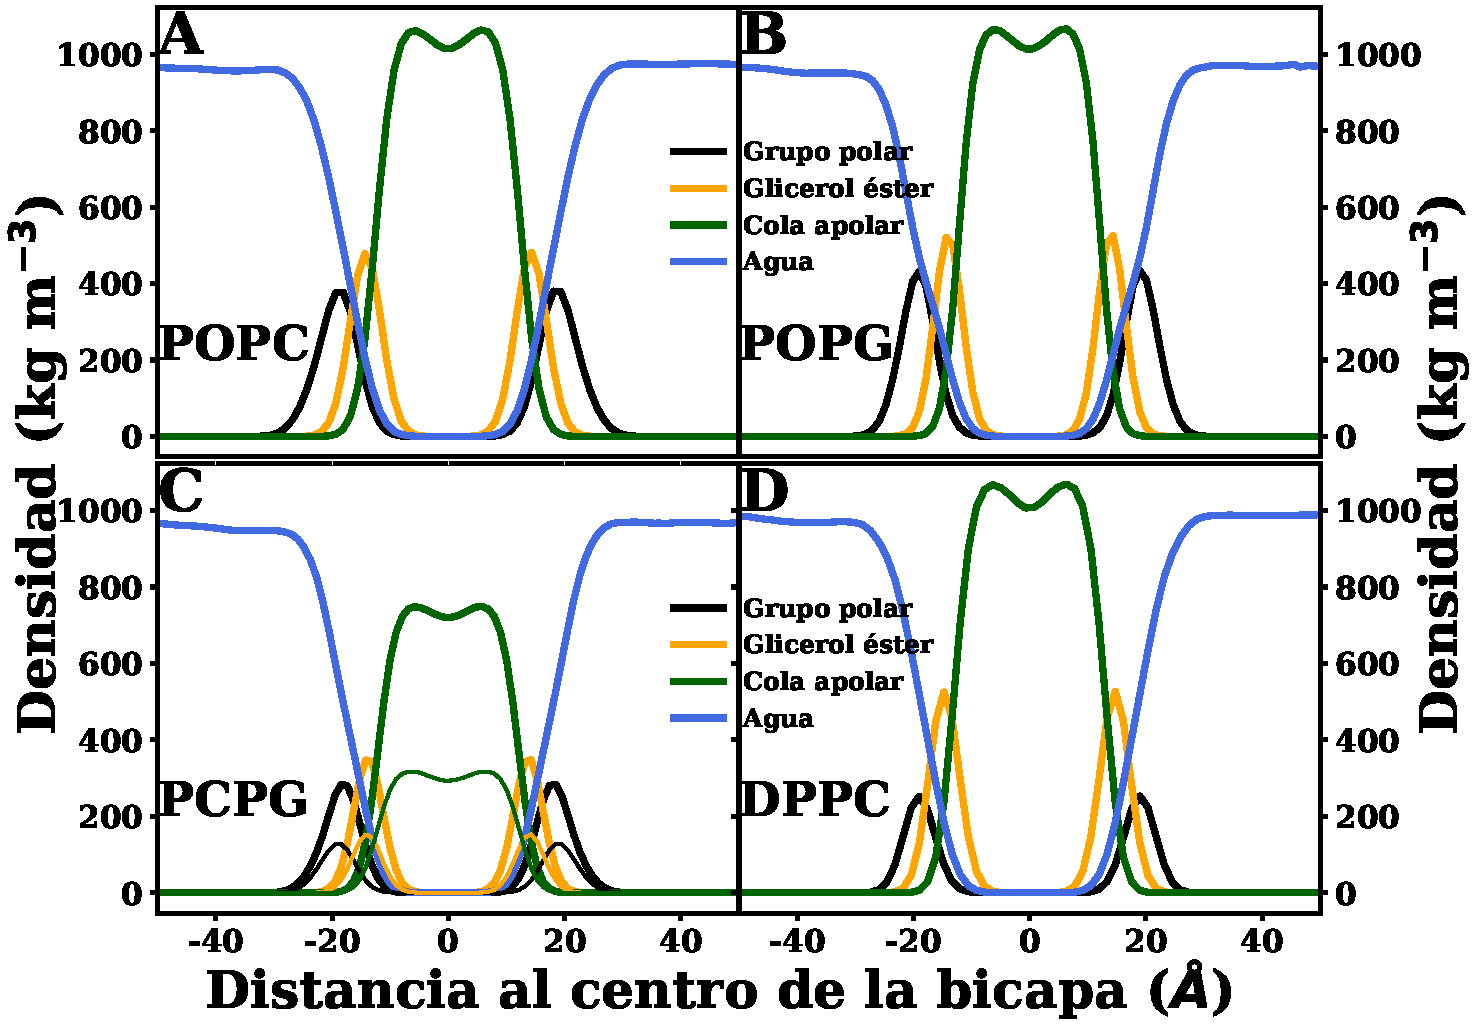
\includegraphics[width=1\linewidth, height=0.8\textheight, keepaspectratio]{fig/02_dm/density_all.pdf} 
	\caption[]{Distrubuciónd e densidad de grupos  \textbf{a-b-c-d)} POPC, DPPC y PCPG}
      \index{density}
    \label{fig:densidad}
\end{figure}
%%%%%%%%%%%%%%%%%%%%%%% Fin %%%%%%%%%%%%%%%%%%%%%%%%


%%%%%%%%%%% Figura %%%%%%%%%%%%
\begin{figure}[H]
    \centering
    \begin{subfigure}[t]{0.45\textwidth}
        \centering
        \subcaption{}
        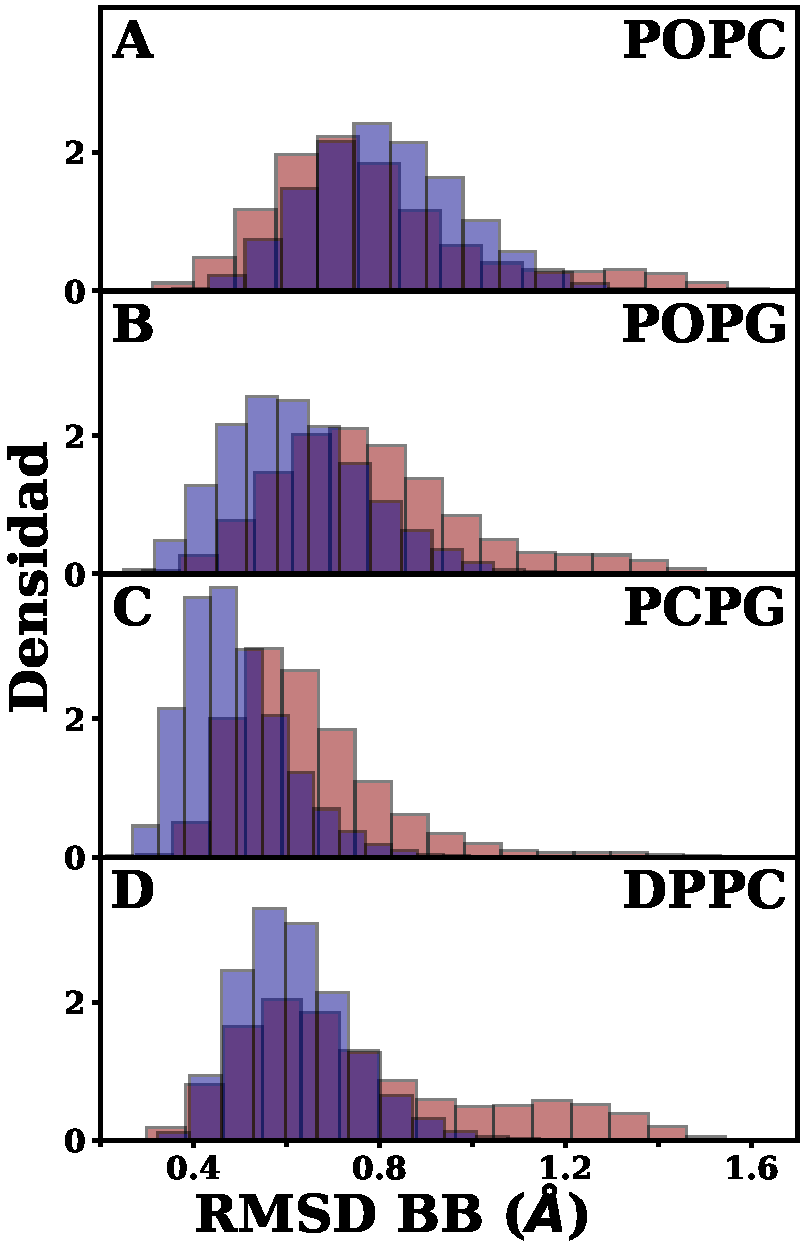
\includegraphics[width=1\linewidth, height=0.99\textheight, keepaspectratio]{fig/02_dm/rmsd_all.pdf} 
    \end{subfigure}
    \begin{subfigure}[t]{0.45\textwidth}
        \centering
        \subcaption{}
        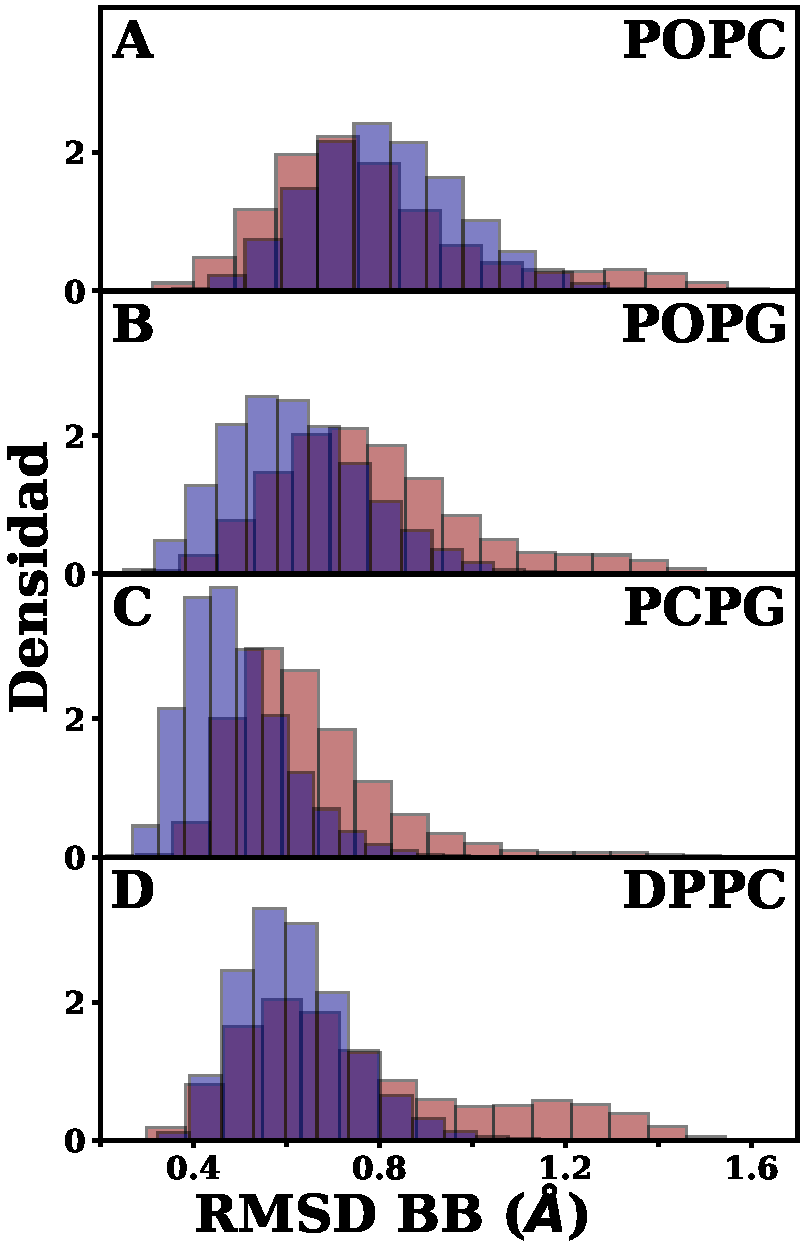
\includegraphics[width=1\linewidth, height=0.99\textheight, keepaspectratio]{fig/02_dm/rmsd_all.pdf}     
    \end{subfigure}
    
\caption[Histograma del RMSD  y \hl{FMSF} de los C$_\alpha$ del dominio transmenbrana $\alpha$IIb/$\beta$3]{Histograma del RMSD  y \hl{FMSF} de los C$_\alpha$ del dominio transmenbrana del dímero $\alpha$IIb/$\beta$3. En cada panel el color rojo y azul representan el péptido $\alpha$IIb y $\beta$3, respectivamente.}
        \index{rmsdf}
    \label{fig:rmsdf}
\end{figure}
%%%%%%%%%%%%%%%%%%%%%%% Fin %%%%%%%%%%%%%%%%%%%%%%%%


%%%%%%%%%%% Figura %%%%%%%%%%%%
\begin{figure}[H]
 \centering
	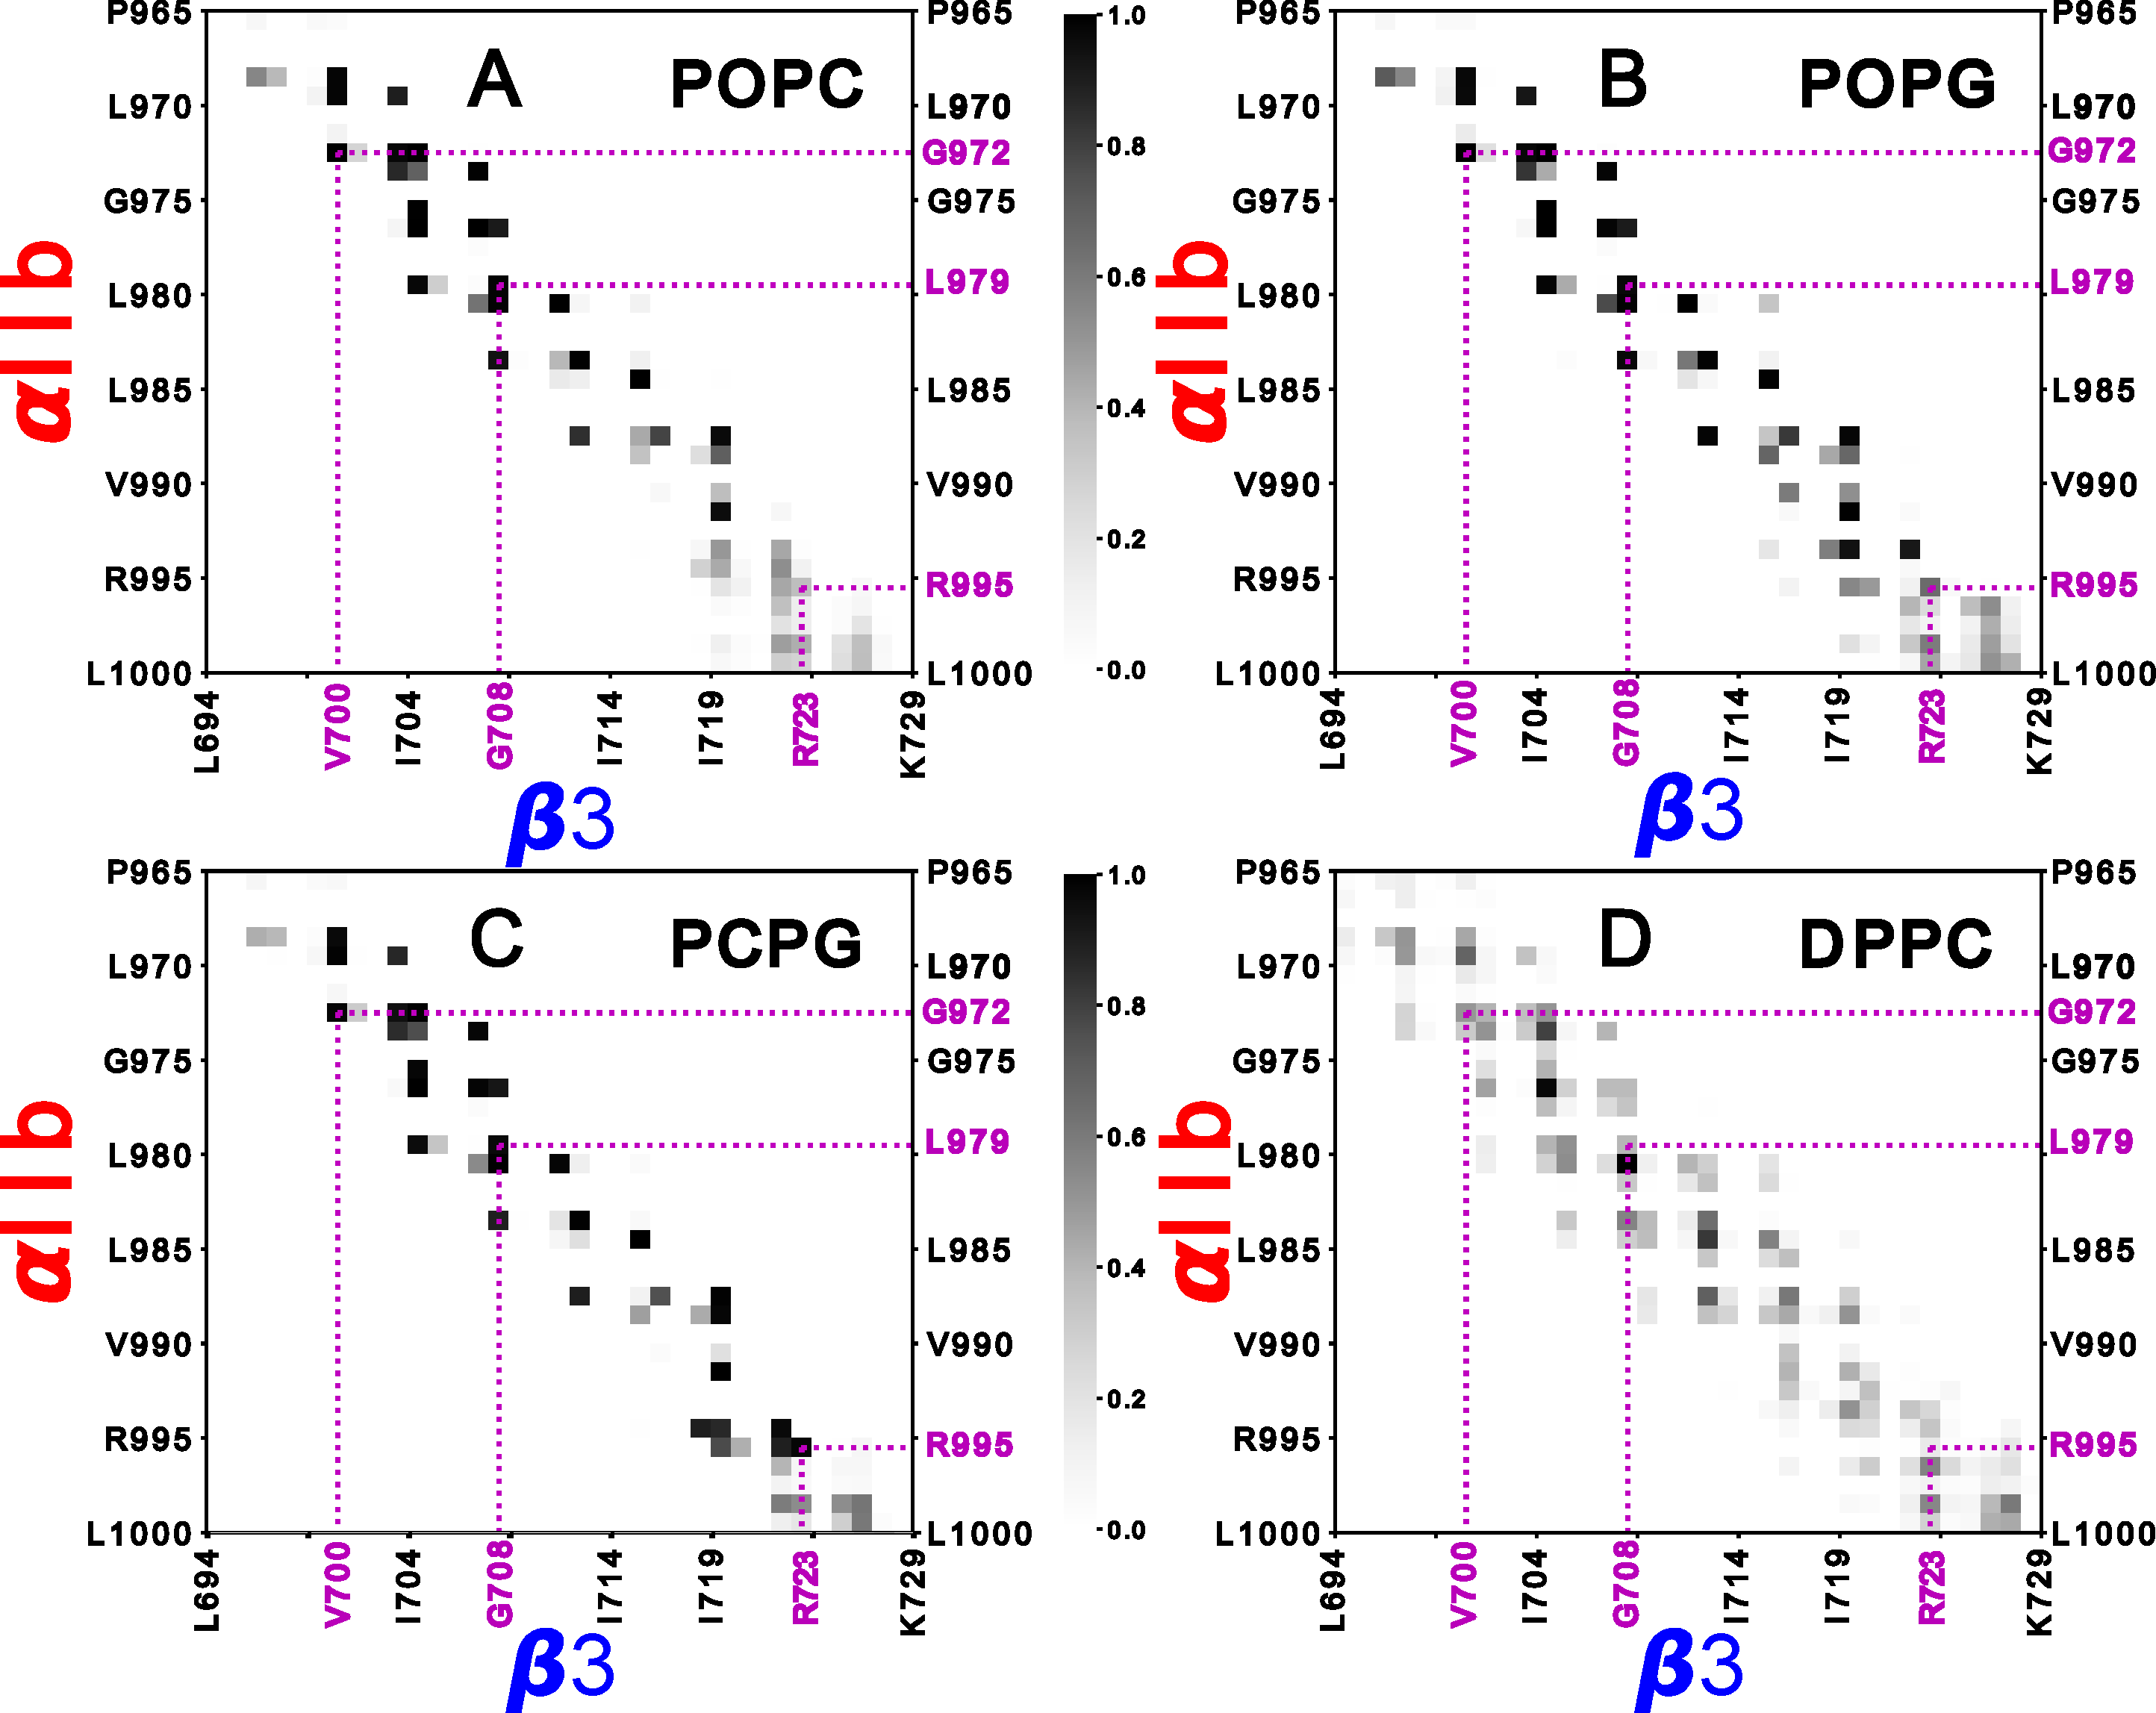
\includegraphics[width=1\linewidth, height=0.8\textheight, keepaspectratio]{fig/02_dm/contact_map2.pdf}
	\caption{Distrubuciónd e densidad de grupos  \textbf{b-c-d)} POPC, DPPC y PCPG}
        \index{headmap}
    	\label{fig:headmap}
\end{figure}

%%%%%%%%%%%%%%%%%%%%%%% Fin %%%%%%%%%%%%%%%%%%%%%%%%



%%%%%%%%%%% Figura %%%%%%%%%%%%
\begin{figure}[H]
    \centering
	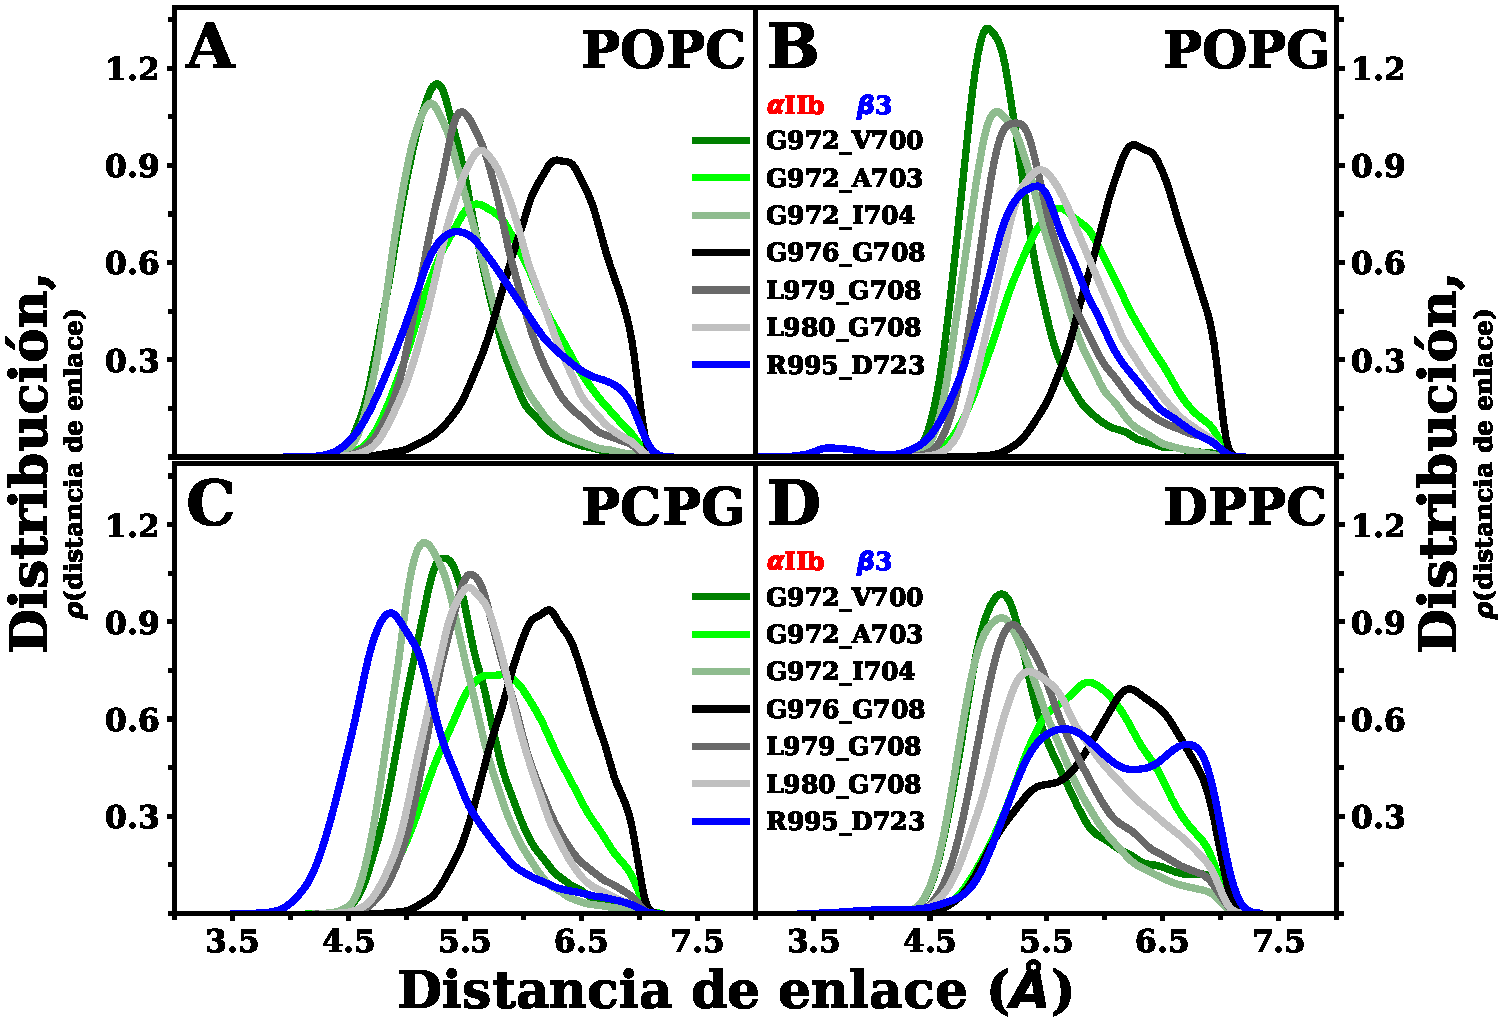
\includegraphics[width=1\linewidth, height=0.99\textheight, keepaspectratio]{fig/02_dm/distance_contacts_all.pdf} 
	\caption{Distribución de densidad de contactos residuos de interés entre heterodímero}
      \index{contac}
    \label{fig:contac}
\end{figure}
%%%%%%%%%%%%%%%%%%%%%%% Fin %%%%%%%%%%%%%%%%%%%%%%%%


%%%%%%%%%%% Figura %%%%%%%%%%%%
\begin{figure}[H]
    \centering
	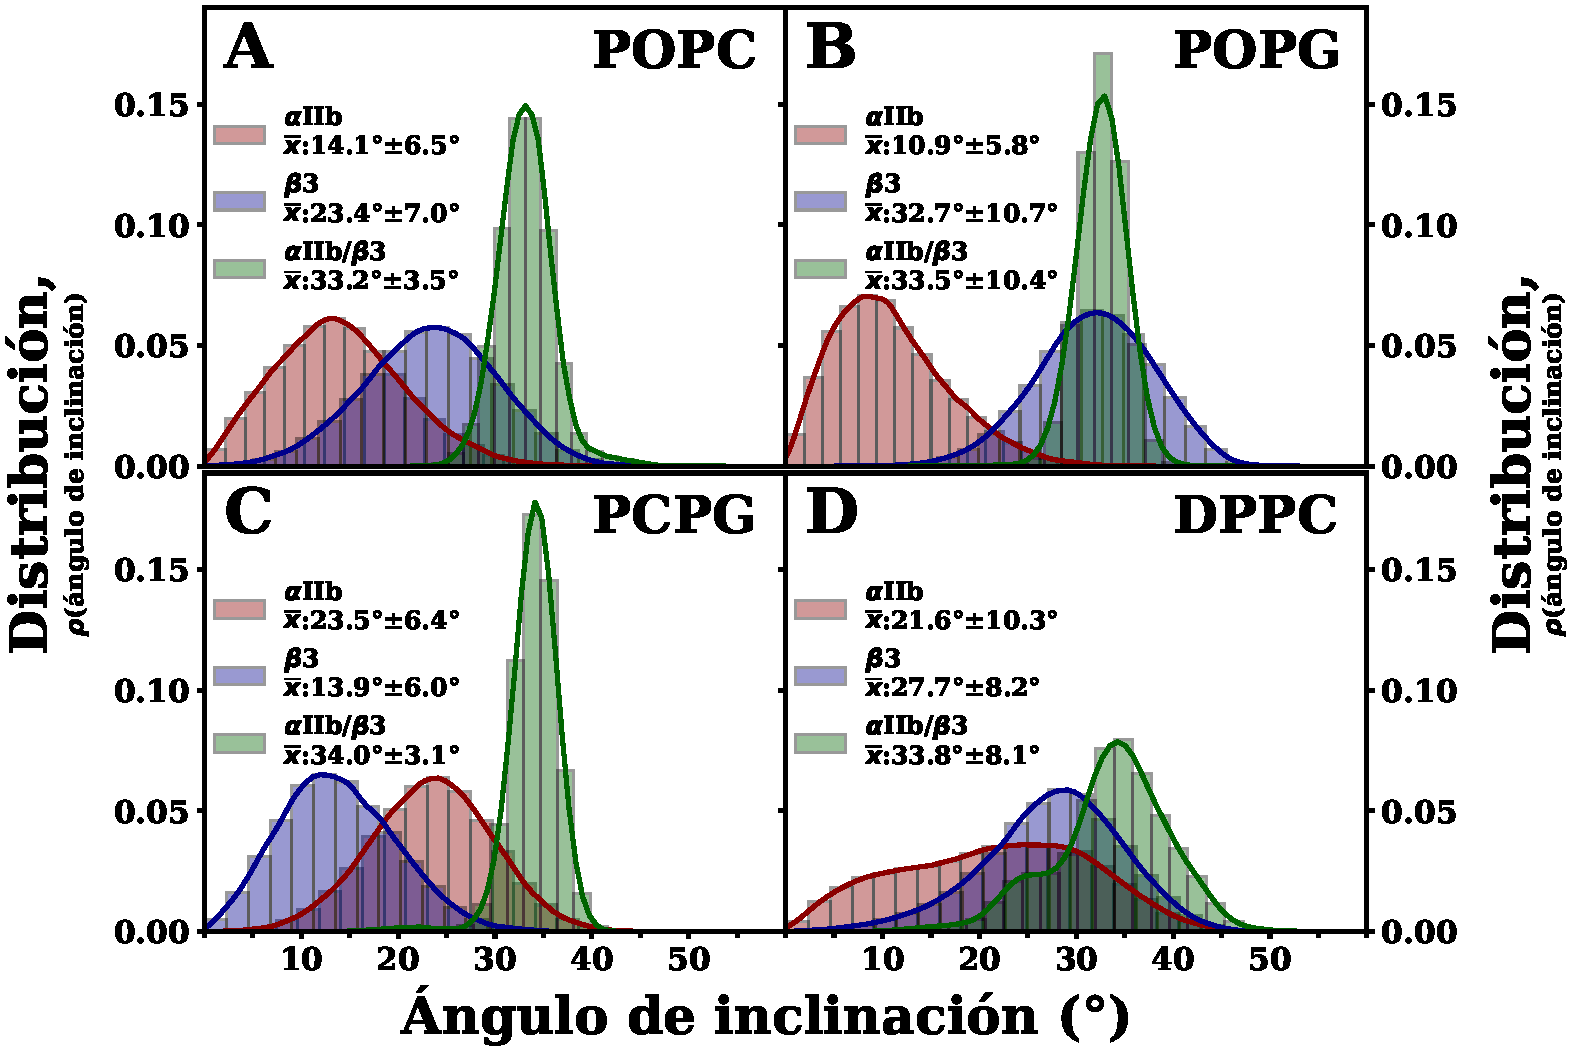
\includegraphics[width=1\linewidth, height=0.8\textheight, keepaspectratio]{fig/02_dm/angles.pdf} 
	\caption[Inclinación respecto a la normal de la bicapa para segmento transmembrana y el ángulo de cruce $\alpha$IIb/$\beta$3]{Inclinación respecto a la normal de la bicapa para segmento transmembrana y el ángulo de cruce $\alpha$IIb/$\beta$3.}
      \index{angles}
    \label{fig:angles}
\end{figure}
%%%%%%%%%%%%%%%%%%%%%%% Fin %%%%%%%%%%%%%%%%%%%%%%%%




%%%%%Tabla resumen membranas%%%%
\begin{table}[h!]
  \begin{center}
%  \centering
%  \captionsetup{justification=centering}  % Center the caption
  \begin{threeparttable}
\centering
    \caption{Área molecular por lípido (APL), parámetro de orden  (S\textbf{\LARGE{$_{cc}$}}) y espesor de membrana durante los 4.5 $\mu$s de simulación. Todos los valores tienen un margen de error de 0.01.}
    \label{tab:parame_lipid}
    \begin{tabular}{l| c c c c}
      \toprule % <-- Toprule here
		Parámetro 					&  POPC	& POPG 	& PCPG 	& DPPC \\ 
      \midrule % <-- Midrule here
		APL (Å\textsuperscript{2}) & 72 	& 73 	& 72 	& 69 \\ 

		S\textbf{\LARGE{$_{cc}$}} 					& 0.52 	& 0.53 	& 0.54	& 0.56 \\ 

		Espesor (Å) 					& 38 	& 34 	& 36 	& 36 \\ 
      \bottomrule % <-- Bottomrule here
    \end{tabular}
    \end{threeparttable}
  \end{center}
\end{table}
%%%%Fin tabla#%%%%%%%%%

%%%%%%%%%%% Figura %%%%%%%%%%%%
\begin{figure}[H]
    \centering
	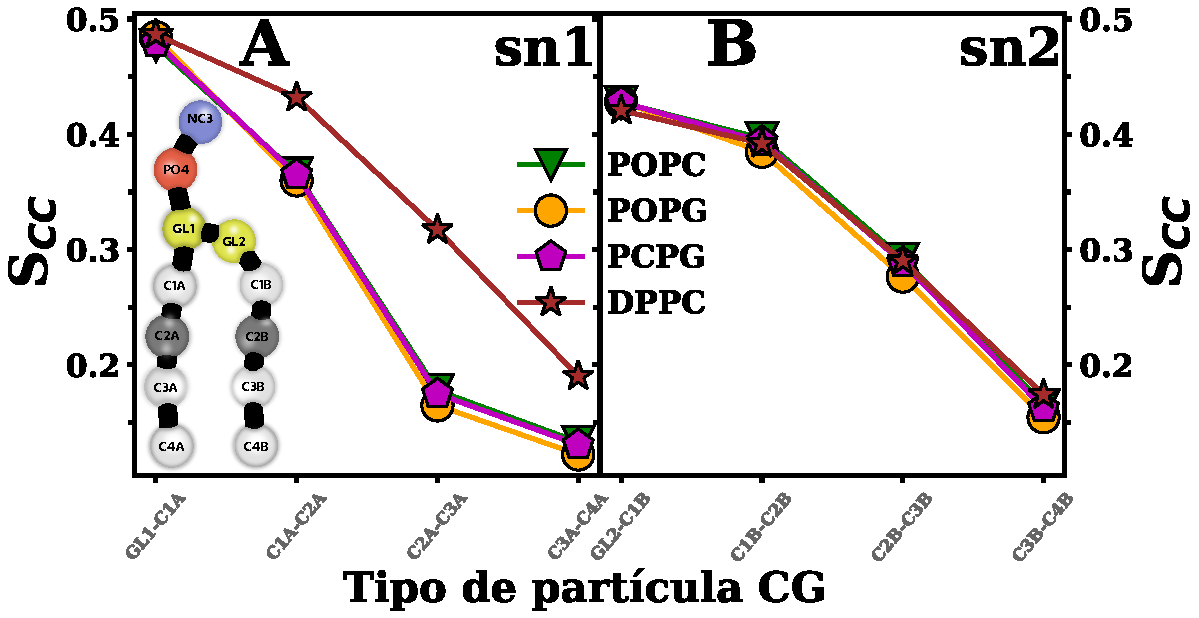
\includegraphics[width=1\linewidth, height=0.99\textheight, keepaspectratio]{fig/02_dm/scc_all.pdf} 
\caption[Parámetro de orden de los lípidos]{Parámetro de orden de los lípidos. Notar que C2A y C2B se resaltan en color diferente porque según el líído que estemos trabajando puede ser D2A y/o D2B}
        \index{areaL}
    \label{fig:scc}
\end{figure}
%%%%%%%%%%%%%%%%%%%%%%% Fin %%%%%%%%%%%%%%%%%%%%%%%%


%%%%%%%%%%% Figura %%%%%%%%%%%%
\begin{figure}[]
    \centering
	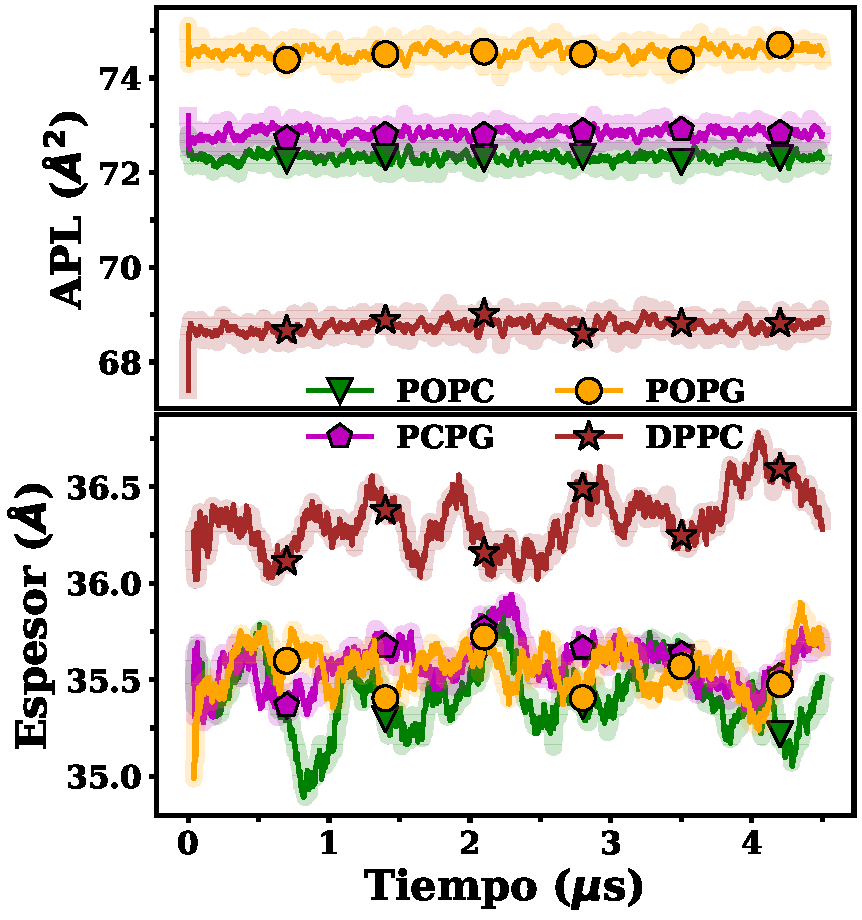
\includegraphics[width=1\linewidth, height=0.99\textheight, keepaspectratio]{fig/02_dm/ApL_zthickness_all.pdf} 
\caption[Área por lípido y espesor de membrana.]{Área por lípido y espesor de membrana.}
        \index{areaL}
    \label{fig:apl_zThick}
\end{figure}
%%%%%%%%%%%%%%%%%%%%%%% Fin %%%%%%%%%%%%%%%%%%%%%%%%


%%%%%%%%%%% Figura %%%%%%%%%%%%
\begin{figure}[H]
    \centering
	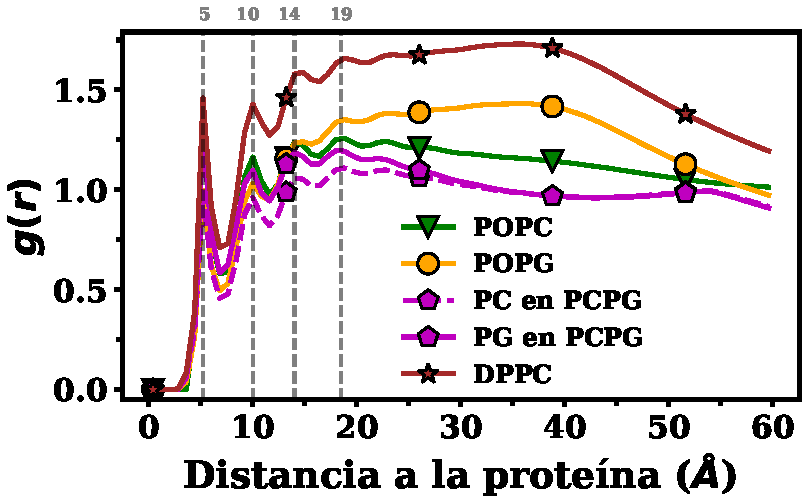
\includegraphics[width=1\linewidth, height=0.99\textheight, keepaspectratio]{fig/02_dm/rdf_all.pdf} 
	\caption[Función de distribución radial] {Función de distribución radial, g(r) para los lípidos respecto al heterodímero $\alpha$IIb/$\beta$3.}
      \index{rdf}
    \label{fig:rdf}
\end{figure}
%%%%%%%%%%%%%%%%%%%%%%% Fin %%%%%%%%%%%%%%%%%%%%%%%%



\begin{table}[H]
\begin{center}
  \begin{threeparttable}
\centering
    \caption[Número de lípidos en contacto con los péptidos.]{Número de lípidos en contacto con los péptidos. Como criterio de contacto se usó un  \textit{cutoff} de 6.0 Å entre el grupo polar PO4 y el centro de masa de los residuos en cada péptido.}
    \label{tab:lipid_pept_contac}
\begin{tabular}{@{}ccccc@{}}
\toprule
                                   & \textbf{POPC}                 & \textbf{POPG}                 & \textbf{PCPG}                 & \textbf{DPPC}                 \\ \cmidrule(l){2-5} 
\multirow{-2}{*}{Péptido} &
  $\overline{x}$\textpm std &
  $\overline{x}$\textpm std &
  $\overline{x}$\textpm std &
  $\overline{x}$\textpm std \\ \midrule
{\color[HTML]{FE0000} $\alpha$IIb} & 19.8\textpm4.8 & 12.1\textpm4.5 & 16.9\textpm5.4 & 13.8\textpm5.3 \\ 
{\color[HTML]{3531FF} $\beta$3}    & 11.1\textpm3.9 & 1.4\textpm4.0  & 13.9\textpm5.4 & 0.9\textpm2.5  \\ \bottomrule
\end{tabular}
\end{threeparttable}
\end{center}
\end{table}



%%%%%%%%%%% Figura %%%%%%%%%%%%
\begin{figure}[H]
    \centering
	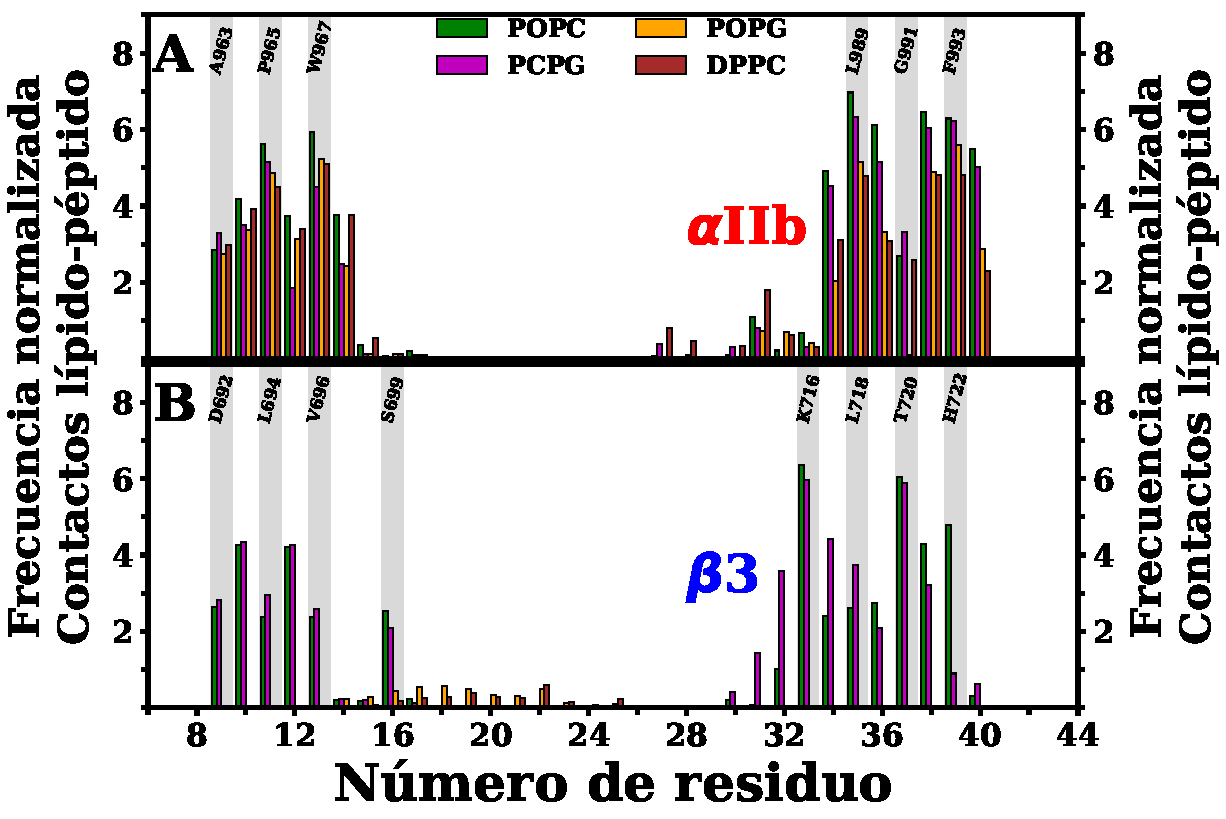
\includegraphics[width=1\linewidth, height=0.99\textheight, keepaspectratio]{fig/02_dm/lipid_pept_contac_all.pdf} 
	\caption[Frecuencia de contactos lípido-residuos durante la dinámica.]{Frecuencia de contactos lípido-residuos durante la dinámica}
      \index{lipid_resid_contact}
    \label{fig:lipid_resID_contac}
\end{figure}
%%%%%%%%%%%%%%%%%%%%%%% Fin %%%%%%%%%%%%%%%%%%%%%%%%